\documentclass{article}

\usepackage{enumitem}
\usepackage{amsmath}
\usepackage{amsfonts}
\usepackage{amssymb}
\usepackage{amsthm}
\usepackage{algorithm}
\usepackage{algorithmic}
\usepackage[margin=0.5in]{geometry}
\usepackage[hidelinks, bookmarks=false]{hyperref}

\usepackage[dvipsnames]{xcolor}

\let\oldemptyset\emptyset
\let\emptyset\varnothing
\newcommand{\R}{\mathbb{R}}
\newcommand{\Rd}{\R^d}

\usepackage{environ}
\NewEnviron{centerframebox}{\begin{center}\fbox{\parbox{0.92\textwidth}{\BODY}}\end{center}}

\title{Discrete and Computational Geometry \\ Assignment 10}
\author{
  \AA{AAAAAAAAAA AAAAAAA}{6} \\
  \href{mailto:\AA{AAAAAAAAAAAAAAAAAAAA}{7}}{\AA{AAAAAAAAAAAAAAAAAAAA}{7}}
  \and
  Ayush Mishra \\
  \href{mailto:s28amish@uni-bonn.de}{s28amish@uni-bonn.de}
}

\usepackage{graphicx}
\graphicspath{{./} {img/}}

\usepackage{titlesec}
\titleformat{\section}
  {\normalfont\Large\bfseries}{Problem \thesection : }
  {0em}{\mdseries}

\begin{document}
  \maketitle
  \begin{center}
    { \bfseries Deadline: 17 Jan 2025, 23:55 }
  \end{center}

  \section{}
  \begin{centerframebox}
    Consider the points $p_1 = (0.05, 0.68)$, $p_2 = (0.07, 0.68)$, $p_3 = (0.12, 0.55)$, $p_4 = (0.3, 0.36)$, $p_5 = (0.63, 0.01)$, $p_6 = (0.68, 0.01)$ as depicted in Figure 1 on the next page.
    Find the WSPD of this point set with separation ratio $s = 3$, which is obtained by the construction algorithm presented in class.
  \end{centerframebox}
  First we must construct a compressed quadtree for our set of points $P = \{p_1,\dots,p_6\}$.
  \begin{center}
    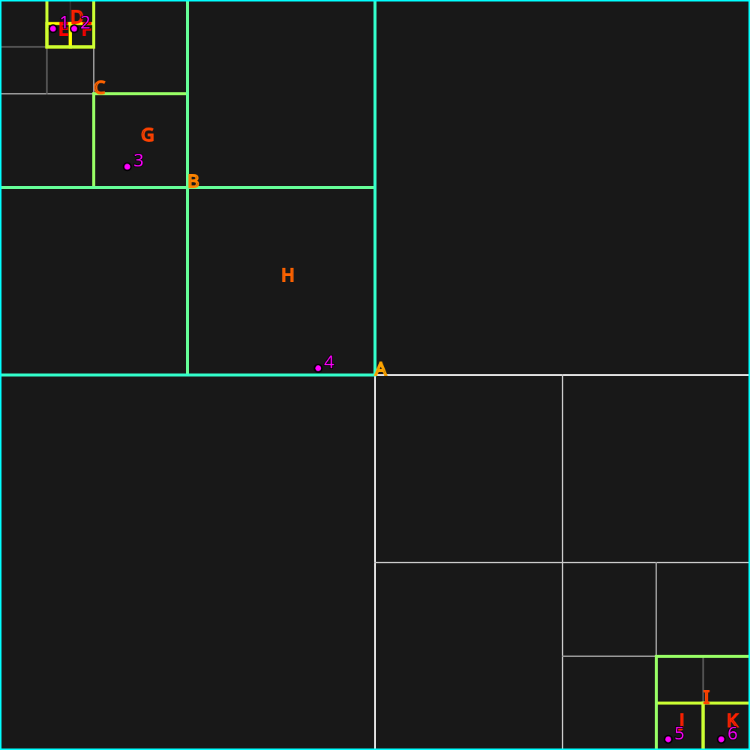
\includegraphics[width=.7\textwidth]{quadtree}

    Figure 1: The quadtree for the set $P$. The cubes are labeled $A$ through $K$.
  \end{center}
  This image also contains the lines for the uncompressed quadtree, to make it easier to see what's going on.

  When constructing the WSPD by hand, we need to visually compare if the two cubes are $s$-well-separated or not.
  For our value of $s=3$, it is easiest to imagine a cube $1.5$ times larger than the larger cube, centered around it, and see if that cube intersects the smaller cube (or the point) we're testing the $s$-well-separated-ness with.

  First call is to the root cube, $\texttt{WellSeparatedPairDecomposition}(A)$.
  Cube $A$ has only tow children: $B$ and $I$.
  They are not well separated, so recurse into cube $B$ and consider the pairs $\{C, I\}$ and $\{H, I\}$.
  $H$ is a leaf node, so when comparing the well-separated-ness, we need to actually take only the point $p_4$.
  Thus both pairs $\{C, I\}$ and $\{H, I\}$ are outputted.
  However we also need to convert the cubes back into point sets:
  the actual pairs in the WSPD end up being $\{\{p_4\}, \{p_5, p_6\}\}$ and $\{\{p_1, p_2, p_3\}, \{p_5, p_6\}\}$.

  Now for a more compact description:
  \begin{itemize}
    \item $\texttt{WellSeparatedPairDecomposition}(A)$
    \begin{itemize}
      \item $\texttt{AddWellSeparatedPairs}(B, I)$ not well separated
      \begin{itemize}
        \item $\texttt{AddWellSeparatedPairs}(C, I)$ are well separated. Output $\{\{p_1, p_2, p_3\}, \{p_5, p_6\}\}$
        \item $\texttt{AddWellSeparatedPairs}(H, I)$ are well separated, because $H$ only contains $p_4$. Output $\{\{p_4\}, \{p_5, p_6\}\}$
      \end{itemize}
    \end{itemize}
    \item $\texttt{WellSeparatedPairDecomposition}(B)$
    \begin{itemize}
      \item $\texttt{AddWellSeparatedPairs}(C, H)$ not well separated
      \begin{itemize}
        \item $\texttt{AddWellSeparatedPairs}(D, H)$ are well separated. Output $\{\{p_4\}, \{p_1, p_2\}\}$
        \item $\texttt{AddWellSeparatedPairs}(G, H)$ are well separated. Output $\{\{p_4\}, \{p_3\}\}$
      \end{itemize}
    \end{itemize}
    \item $\texttt{WellSeparatedPairDecomposition}(C)$
    \begin{itemize}
      \item $\texttt{AddWellSeparatedPairs}(D, G)$ are well separated, because $G$ is a leaf. Output $\{\{p_3\}, \{p_1, p_2\}\}$
    \end{itemize}
    \item $\texttt{WellSeparatedPairDecomposition}(D)$
    \begin{itemize}
      \item $\texttt{AddWellSeparatedPairs}(E, F)$ are well separated, because they are both leaves. Output $\{\{p_1\}, \{p_2\}\}$
    \end{itemize}
    \item $\texttt{WellSeparatedPairDecomposition}(I)$
    \begin{itemize}
      \item $\texttt{AddWellSeparatedPairs}(J, K)$ are well separated, because they are both leaves. Output $\{\{p_5\}, \{p_6\}\}$
    \end{itemize}
  \end{itemize}
  Calls to \texttt{WellSeparatedPairDecomposition} have been omitted for leaf nodes.

  \newpage
  \section{}
  \begin{centerframebox}
    For any $p \in \mathbb{R}^2$, $r > 0$, let $B(p, r)$ be the Euclidean ball of radius $r$, centered at $p$. Consider a set $P$ of $n$ points in $\mathbb{R}^2$, stored in a compressed quadtree. Design an algorithm which, given a query point $q \in \mathbb{R}^2$, radius $r > 0$, and approximation parameter $1 \geq \epsilon > 0$, returns an integer $m$ such that

\[
|B(q, r) \cap P | \leq m \leq |B(q, (1 + \epsilon)r) \cap P |.
\]

You can assume that the compressed quadtree of $P$ stores for each node the number of leaves of its subtree. The query algorithm must be adaptive to $\epsilon$, meaning that larger values of $\epsilon$ should lead to faster running time. Analyse the running time of your algorithm.
  \end{centerframebox}

  To solve this problem, we need to count points in a query ball while allowing some approximation. The key insight is that we can use the compressed quadtree to efficiently process regions of space based on their relationship to the query balls.

\paragraph{Algorithm} For a cube $C$, let $\text{corners}(C)$ be its set of corners. Define:
\[
\text{mindist}(C,q) = \min_{c \in \text{corners}(C)} \|c-q\|
\]
\[
\text{maxdist}(C,q) = \max_{c \in \text{corners}(C)} \|c-q\|
\]

These determine tight bounds on distances to any point in $C$: by convexity of Euclidean distance and of cubes, for any point $p$ in $C$, we have $\text{mindist}(C,q) \leq \|p-q\| \leq \text{maxdist}(C,q)$. By the problem assumption, for each node $u$, $\text{count}(u)$ gives the number of points stored in the subtree rooted at $u$. Our algorithm is:

\begin{algorithmic}[1]
\STATE \textbf{procedure} CountInBall(node $u$, point $q$, radius $r$, $\epsilon$)
\STATE Let $C = \text{Cube}(u)$
\STATE // Case 1: Cube entirely inside inner ball
\IF{$\text{maxdist}(C,q) \leq r$}
   \STATE \textbf{return} $\text{count}(u)$
\ENDIF
\STATE // Case 2: Cube entirely outside outer ball
\IF{$\text{mindist}(C,q) > (1+\epsilon)r$}
   \STATE \textbf{return} 0
\ENDIF
\STATE // Case 3: Leaf case
\IF{$u$ is a leaf}
   \STATE Let $p$ be the point stored at $u$
   \STATE \textbf{return} $[\|p-q\| \leq r]$ \COMMENT{where $[P]$ is 1 if predicate $P$ is true, 0 otherwise}
\ENDIF
\STATE // Case 4: Recursive case
\STATE result $\gets 0$
\FOR{$v \in \text{children}(u)$}
   \STATE result $\gets$ result + CountInBall($v,q,r,\epsilon$)
\ENDFOR
\STATE \textbf{return} result
\end{algorithmic}

\paragraph{Correctness} We need to prove that our output $m$ satisfies:
\[
|B(q, r) \cap P| \leq m \leq |B(q, (1+\epsilon)r) \cap P|
\]

For the lower bound, consider any point $p \in B(q,r) \cap P$. This point must be counted exactly once by our algorithm:
\begin{itemize}
   \item If $p$ is in a cube $C$ with $\text{maxdist}(C,q) \leq r$, then $\|p-q\| \leq r$ and $p$ is counted in Case 1
   \item Otherwise, we eventually reach $p$'s leaf node, where $\|p-q\| \leq r$ implies $p$ is counted in Case 3
\end{itemize}
The quadtree structure ensures no point is counted twice since each point appears in exactly one leaf node, and internal nodes partition the point set. Therefore, $m \geq |B(q,r) \cap P|$.

For the upper bound, we show that any point $p$ counted by our algorithm must lie in $B(q,(1+\epsilon)r)$:
\begin{itemize}
   \item Points counted in Case 1 are in cubes $C$ with $\text{maxdist}(C,q) \leq r$, so they lie in $B(q,r)$ and thus in $B(q,(1+\epsilon)r)$
   \item Points counted in Case 3 have $\|p-q\| \leq r$, so they also lie in $B(q,(1+\epsilon)r)$
   \item Case 2 explicitly excludes any cube $C$ with $\text{mindist}(C,q) > (1+\epsilon)r$, so no points outside $B(q,(1+\epsilon)r)$ can be counted
\end{itemize}
Therefore, $m \leq |B(q,(1+\epsilon)r) \cap P|$.

\paragraph{Running Time Analysis} for the running time analysis we need to analyze the counting of how many nodes our algorithm processes. Consider three regions:

\begin{enumerate}
    \item Nodes entirely inside $B(q,r)$ - processed in constant time via Case 1
    \item Nodes entirely outside $B(q,(1+\epsilon)r)$ - processed in constant time via Case 2
    \item Nodes intersecting the annulus between these balls - require recursive processing
\end{enumerate}

At each level $i$ of the quadtree where cells have diameter $d_i = \delta/2^i$ (where $\delta$ is the diameter of the root cube), we only need to analyze the nodes in region 3, as nodes in regions 1 and 2 contribute only $O(1)$ to the running time.

This annulus has width $\epsilon r$ and radius $r$, giving it a circumference of $O(r)$ and total area:
\[
\pi((1+\epsilon)r)^2 - \pi r^2 = \pi r^2(2\epsilon + \epsilon^2) = O(\epsilon r^2)
\]

A cell of diameter $d_i$ that intersects the annulus must have its center within distance $d_i$ of the annulus. Therefore, the intersecting cells cover a region of area $O(\epsilon r^2)$. Since cells at level $i$ are disjoint and each has area $\Theta(d_i^2)$, the number of intersecting cells at level $i$ is $O(\epsilon r^2/d_i^2)$.

The total running time is thus bounded by:
\[
T(n) = O\left(\sum_{i=0}^h \min\left\{n, \frac{\epsilon r^2}{d_i^2}\right\}\right) = O\left(\sum_{i=0}^h \min\left\{n, \epsilon r^2 \cdot \frac{4^i}{\delta^2}\right\}\right)
\]

From Lemma 17.6 in the lecture, we know that $h \in O(\log(\phi(P)))$, where $\phi(P)$ is the spread of $P$. The sum is dominated by either $n$ terms (when $n$ is small) or by its largest term with $\epsilon$ (when $1/\epsilon$ is small), giving us our final bound:
\[
T(n) = O\left(\min\left\{n, \frac{1}{\epsilon}\right\}\log(\phi(P))\right)
\]

This shows that our algorithm is adaptive to $\epsilon$ as required - larger values of $\epsilon$ lead to faster running times since we process fewer nodes in the annulus region.

The algorithm uses $O(1)$ additional space beyond the input quadtree, as it only needs constant space per recursive call and the recursion depth is $O(\log(\phi(P)))$. The required count values for each node can be precomputed in $O(n)$ time during quadtree construction using a simple bottom-up traversal.

  \section{}
  \begin{centerframebox}
    Prove the following statement (Lemma 18.5): Let $P$ be a set of $n$ points in $\R^d$. For any two
    distinct points $p, q \in P$, the algorithm WellSeparatedPairDecomposition from the lecture
    outputs exactly one $s$-well-separated pair that covers $\{p, q\}$.
  \end{centerframebox}
  Consider the node $a$ which is the lowest common ancestor of $p$ and $q$ in the quadtree.
  We know that the algorithm must have called $\texttt{WellSeparatedPairDecomposition}(a)$, because it calls that for every node in the tree.
  And it would've called $\texttt{AddWellSeparatedPairs}(p', q')$ with $p'$ and $q'$ being the branches leading to $p$ and $q$ respectively.
  If they are well separated, the pair $\{p', q'\}$ is added to the WSPD, and if not, we go down into all of the children.
  Here we can ignore all children that do not contain either $p$ or $q$.
  On each level of the recursion, there will be exactly one call to \texttt{AddWellSeparatedPairs} that contains both $p$ and $q$.
  This will continued until a well separated pair of cubes is found, or we reach the bottom and just return $\{\{p\}, \{q\}\}$ as a pair.

  No pair coming from other calls to \texttt{WellSeparatedPairDecomposition} can contain $p$ and $q$ on different sides.
  Calls for nodes bellow $a$ will only generate pairs that don't contain both $p$ and $q$.
  And calls for nodes above $a$ will have $p$ and $q$ on the same side.
  So the pair can only be outputted once.

  \section{}
  \begin{centerframebox}
    Define the weight of a WSPD \(\{ \{A_1, B_1\}, \ldots, \{A_m, B_m\} \}\) as the quantity
    \[ \sum_{i=1}^m |A_i| + |B_i| \]
    Show that there exists a set of \(n\) points in \(\R^1\), such that any WSPD with separation ratio at least 2 has weight \(\Omega(n^2)\).
  \end{centerframebox}
  To construct this set of points, we first divide it into two equal sets $A$ and $B$ of $n/2$ points each.
  Points in set $A$ are all placed inside a small ball of radius $\epsilon$ centered at the origin.
  The remaining points in $B$ are all spaced a distance $k \cdot 2^i$ apart (for the $i$-th point in $B$), with $k \gg \epsilon$, starting at distance $k-\epsilon$ from the $A$ ball.

  This arrangement makes in so each point in $B$ needs to have a separate pair with the set $A$.
  Trying to group any two points in $B$ together will result in a ball that is not well separated from $A$.
  The distance to $A$ will be at least the ball's diameter, and this is not allowed, as our separation factor $s \geq 2$.

  This way the WSPD must include $n/2$ pairs of the form $\{A, \{p_i\}\}$ for all $p_i \in B$.
  Each one of those pairs contributes $n/2+1$ to the weight of the decomposition,
  and in total the weight must be at least $n/2 \cdot (n/2+1)$ which is in $\omega(n^2)$.

  To prove the upper bound we just consider the simple WSPD constructed by taking each possible pair of points.
  It has size $O(n^2)$ and also weight $O(n^2)$.
  Thus the bound is $\Omega(n^2)$.

\end{document}
